\documentclass[11pt, fleqn]{article}

\usepackage{amsmath}
\usepackage{amssymb}
\usepackage{amsthm}
\usepackage{mathtools}
\usepackage{hyperref}
\usepackage{ulem}
\usepackage{enumitem}
\usepackage[left=0.75in, right=0.75in, bottom=0.75in, top=1.0in]{geometry}
\usepackage{floatrow}
\usepackage{graphicx}
\usepackage[export]{adjustbox}
\usepackage{sectsty}
\sectionfont{\centering}

\usepackage{multirow}
\usepackage{multicol}

\usepackage[dvipsnames]{xcolor}

\usepackage[perpage]{footmisc}

\usepackage{fancyhdr}
\pagestyle{fancy}
\fancyhf{}
\lhead{190100044}
\rhead{CS 252: Lab 5}
\renewcommand{\footrulewidth}{1.0pt}
\cfoot{Page \thepage}

\setlength{\parindent}{0em}

\title{\vspace{-4em}CS 252: Lab 5}
\author{Devansh Jain, 190100044}
\date{\today}

\begin{document}

% \pagenumbering{gobble}
\maketitle
\tableofcontents
\thispagestyle{empty}
\setcounter{page}{0}


\newpage 
\section*{Question 1}
\addcontentsline{toc}{section}{Question 1}
\setcounter{equation}{0}

\subsection*{a.}
\addcontentsline{toc}{subsection}{a.}

For default parameters (\texttt{dataRate} = 10.0Mbps),\\

Throughput for Flow 1 (Node n1 $\rightarrow$ Node n0): \\
9.7141 Mbps (RTS/CTS disabled), 10.1113 Mbps (RTS/CTS enabled) \\

Throughput for Flow 2 (Node n2 $\rightarrow$ Node n0): \\
9.3780 Mbps (RTS/CTS disabled), 10.0960 Mbps (RTS/CTS enabled) \\

Total Channel Throughput: \\
19.0921 Mbps (RTS/CTS disabled), 20.2073 Mbps (RTS/CTS enabled) \\

\subsection*{b.}
\addcontentsline{toc}{subsection}{b.}

Channel data rate is 54 Mbps.

\begin{figure}[H]
    \centering
    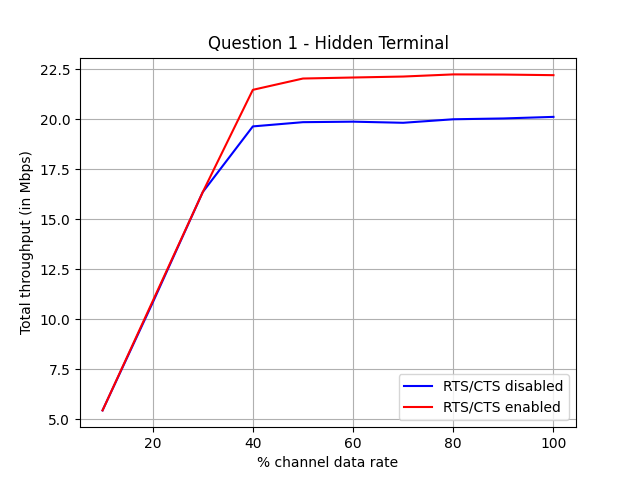
\includegraphics{q1.png}
\end{figure}

\begin{table}[H]
    \centering
    \begin{tabular}{||c|c||c|c||}
         \hline
         \multirow{2}{*}{Total Data Rate Offered} & \multirow{2}{*}{\texttt{dataRate}} & \multicolumn{2}{c||}{Total Throughput} \\
         & & RTS/CTS disabled & RTS/CTS enabled \\
         \hline % 10
         10\% of channel date rate & 2.7Mbps & 5.4541 Mbps & 5.4541 Mbps \\
         \hline % 20
         20\% of channel date rate & 5.4Mbps & 10.8344 Mbps & 10.9108 Mbps \\
         \hline % 30
         30\% of channel date rate & 8.1Mbps & 16.3675 Mbps & 16.3675 Mbps \\
         \hline % 40
         40\% of channel date rate & 10.8Mbps & 19.6522 Mbps & 21.4805 Mbps \\
         \hline % 50
         50\% of channel date rate & 13.5Mbps & 19.8636 Mbps & 22.0457 Mbps \\
         \hline % 60
         60\% of channel date rate & 16.2Mbps & 19.8890 Mbps & 22.0967 Mbps \\
         \hline % 70
         70\% of channel date rate & 18.9Mbps & 19.8330 Mbps & 22.1450 Mbps \\
         \hline % 80
         80\% of channel date rate & 21.6Mbps & 20.0087 Mbps & 22.2520 Mbps \\
         \hline % 90
         90\% of channel date rate & 24.3Mbps & 20.0495 Mbps & 22.2444 Mbps \\
         \hline % 100
         100\% of channel date rate & 27.0Mbps & 20.1284 Mbps & 22.2138 Mbps \\
         \hline         
    \end{tabular}
\end{table}

We can see that Total throughput increases with Offered Load and almost flattens to a constant value by the end. \\
We also see that RTS/CTS disabled network has less maximum throughput than RTS/CTS enabled network. \\

\subsection*{c.}
\addcontentsline{toc}{subsection}{c.}
Only Flow 1 (Node n1 $\rightarrow$ Node n0) \\
RTS/CTS disabled: Total throughput saturates at 25.6182 Mbps for \texttt{dataRate} = 35 Mbps. \\
RTS/CTS enabled: Total throughput saturates at 22.6696 Mbps for \texttt{dataRate} = 24 Mbps. \\

We can see that Total throughput increases with Offered Load and almost flattens to a constant value by the end. \\
We also see that RTS/CTS disabled network has more maximum throughput than RTS/CTS enabled network. \\

\subsection*{d.}
\addcontentsline{toc}{subsection}{d.}

\begin{itemize}
    \item Total throughput is less than total data rate offered in all cases.
    \item We can see that Total throughput increases with Offered Load and almost flattens to a constant value by the end, both for two source and one source
    \item We also see that RTS/CTS disabled network has less maximum throughput than RTS/CTS enabled network when we have two sources but has more maximum throughput when we have only one source.
    \item We reach saturation for both cases when total data rate offered is about 40\% of channel data rate.
\end{itemize}

\newpage
\section*{Question 2}
\addcontentsline{toc}{section}{Question 2}
\setcounter{equation}{0}

\subsection*{a.}
\addcontentsline{toc}{subsection}{a.}

Channel data rate is 54 Mbps.

\begin{figure}[H]
    \centering
    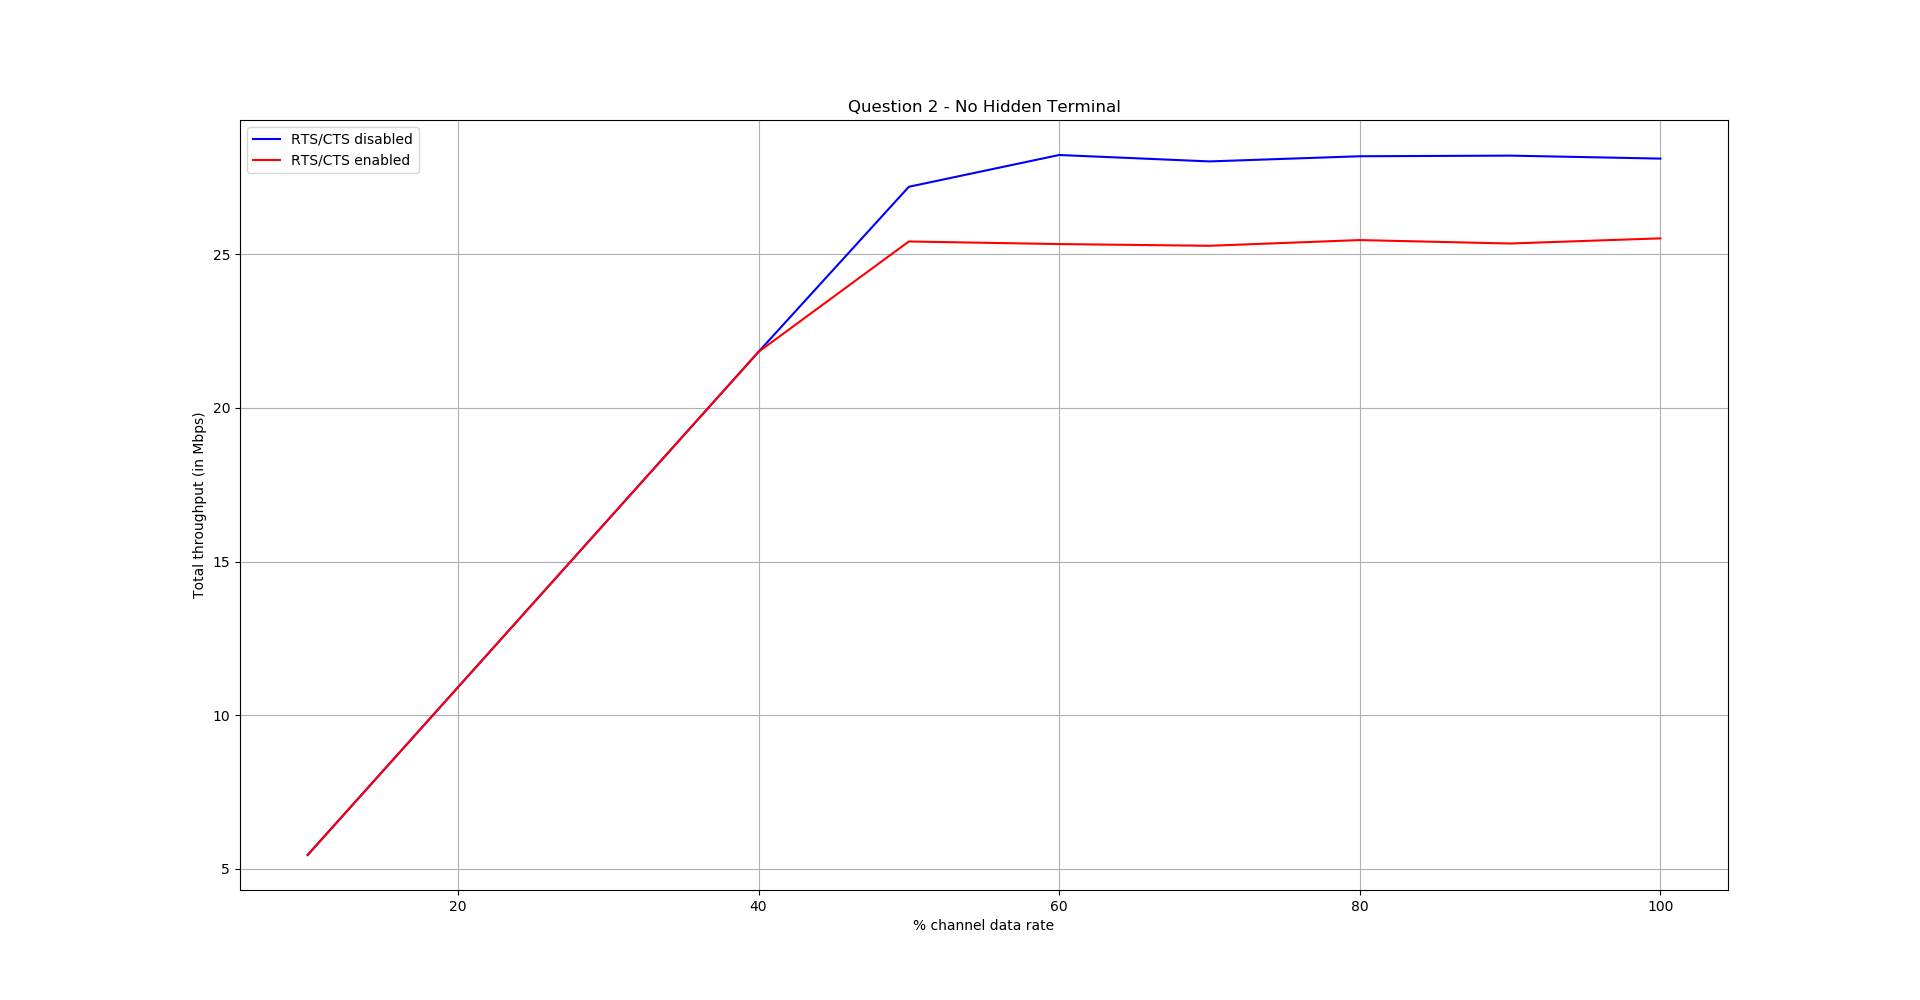
\includegraphics{q2.png}
\end{figure}

\begin{table}[H]
    \centering
    \begin{tabular}{||c|c||c|c||}
         \hline
         \multirow{2}{*}{Total Data Rate Offered} & \multirow{2}{*}{\texttt{dataRate}} & \multicolumn{2}{c||}{Total Throughput} \\
         & & RTS/CTS disabled & RTS/CTS enabled \\
         \hline % 10
         10\% of channel date rate & 2.7Mbps & 5.4541 Mbps & 5.4541 Mbps \\
         \hline % 20
         20\% of channel date rate & 5.4Mbps & 10.9108 Mbps & 10.9108 Mbps \\
         \hline % 30
         30\% of channel date rate & 8.1Mbps & 16.3675 Mbps & 16.3675 Mbps \\
         \hline % 40
         40\% of channel date rate & 10.8Mbps & 21.8242 Mbps & 21.8242 Mbps \\
         \hline % 50
         50\% of channel date rate & 13.5Mbps & 27.1943 Mbps & 25.4145 Mbps \\
         \hline % 60
         60\% of channel date rate & 16.2Mbps & 28.2281 Mbps & 25.3305 Mbps \\
         \hline % 70
         70\% of channel date rate & 18.9Mbps & 28.0193 Mbps & 25.2744 Mbps \\
         \hline % 80
         80\% of channel date rate & 21.6Mbps & 28.1874 Mbps & 25.4603 Mbps \\
         \hline % 90
         90\% of channel date rate & 24.3Mbps & 28.2078 Mbps & 25.3483 Mbps \\
         \hline % 100
         100\% of channel date rate & 27.0Mbps & 28.1110 Mbps & 25.5163 Mbps \\
         \hline         
    \end{tabular}
\end{table}

We can see that Total throughput increases with Offered Load and almost flattens by the end. \\
We also see that RTS/CTS disabled network has more maximum throughput than RTS/CTS enabled network.

\subsection*{b.}
\addcontentsline{toc}{subsection}{b.}

\begin{itemize}
    \item Total throughput is less than total data rate offered in all cases.
    \item We can see that Total throughput increases with Offered Load and almost flattens to a constant value by the end, both for two source and one source
    \item We also see that RTS/CTS disabled network has more maximum throughput than RTS/CTS enabled network.
    \item We reach saturation for both cases when total data rate offered is about 50\% of channel data rate.
    \item The saturation level as compared to Question 1 (where a hidden terminal pair was present) is more for both cases.
\end{itemize}

\newpage 
\section*{Question 3}
\addcontentsline{toc}{section}{Question 3}
\setcounter{equation}{0}

\subsection*{a.}
\addcontentsline{toc}{subsection}{a.}

For default parameters (\texttt{dataRate} = 10.0Mbps),\\

Throughput for Flow 1 (Node A1 $\rightarrow$ Node A2): 10.1088 Mbps (RTS/CTS enabled) \\
Throughput for Flow 2 (Node B1 $\rightarrow$ Node B2): 9.5536 Mbps (RTS/CTS enabled) \\
Throughput for Flow 3 (Node C1 $\rightarrow$ Node C2): 10.0782 Mbps (RTS/CTS enabled) \\

Total Channel Throughput: 29.7406 Mbps (RTS/CTS enabled) \\

\subsection*{b.}
\addcontentsline{toc}{subsection}{b.}

Channel data rate is 54 Mbps.

\begin{figure}[H]
    \centering
    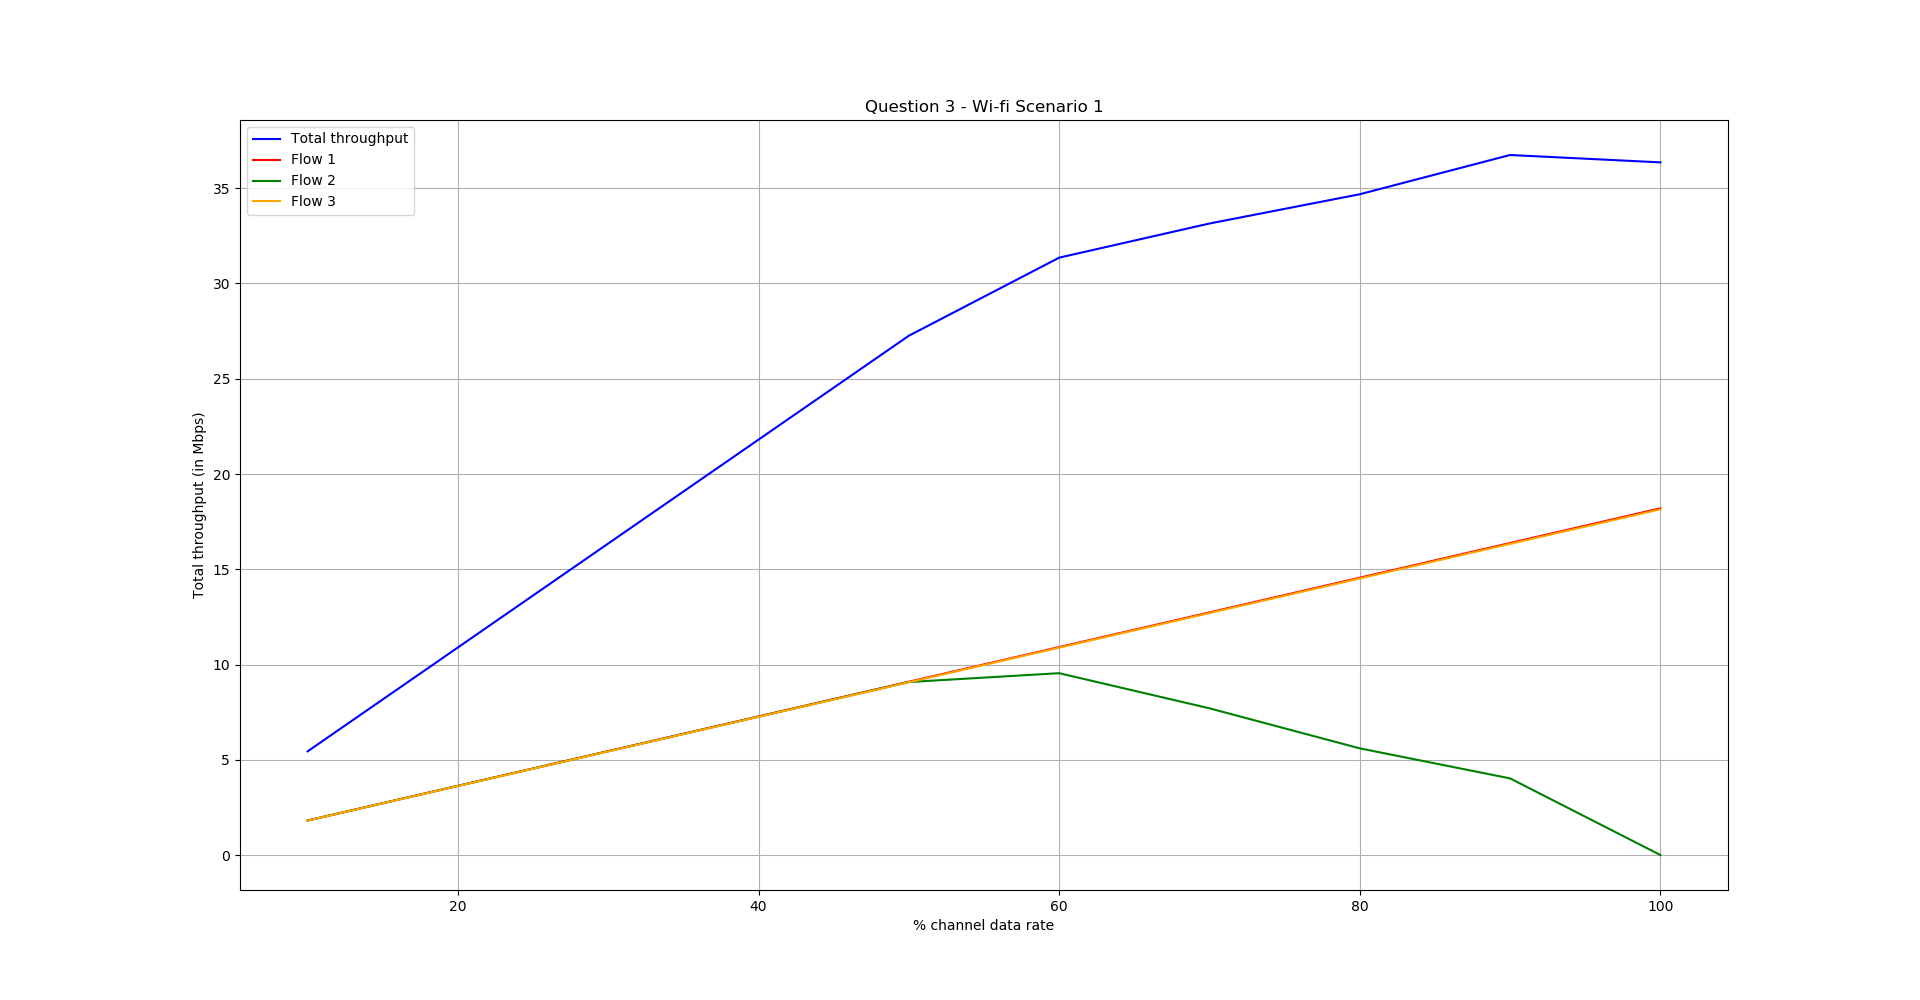
\includegraphics{q3.png}
\end{figure}

\begin{table}[H]
    \centering
    \begin{tabular}{||c|c||c|c|c||c||}
         \hline
         Total Data Rate Offered & \texttt{dataRate} & Flow 1 & Flow 2 & Flow 3 & Total Throughput \\
         \hline % 10
         10\% of channel date rate & 1.8Mbps & 1.8180 Mbps & 1.8155 Mbps & 1.8130 Mbps & 5.4465 Mbps \\
         \hline % 20
         20\% of channel date rate & 3.6Mbps & 3.6386 Mbps & 3.6335 Mbps & 3.6285 Mbps & 10.9006 Mbps \\
         \hline % 30
         30\% of channel date rate & 5.4Mbps & 5.4592 Mbps & 5.4516 Mbps & 5.4440 Mbps & 16.3548 Mbps \\
         \hline % 40
         40\% of channel date rate & 7.2Mbps & 7.2798 Mbps & 7.2671 Mbps & 7.2595 Mbps & 21.8064 Mbps \\
         \hline % 50
         50\% of channel date rate & 9.0Mbps & 9.1004 Mbps & 9.0852 Mbps & 9.0724 Mbps & 27.2580 Mbps \\
         \hline % 60
         60\% of channel date rate & 10.8Mbps & 10.9185 Mbps & 9.5486 Mbps & 10.8879 Mbps & 31.3550 Mbps \\
         \hline % 70
         70\% of channel date rate & 12.6Mbps & 12.7391 Mbps & 7.7050 Mbps & 12.7034 Mbps & 33.1475 Mbps \\
         \hline % 80
         80\% of channel date rate & 14.4Mbps & 14.5597 Mbps & 5.6044 Mbps & 14.5189 Mbps & 34.6830 Mbps \\
         \hline % 90
         90\% of channel date rate & 16.2Mbps & 16.3803 Mbps & 4.0282 Mbps & 16.3344 Mbps & 36.7429 Mbps \\
         \hline % 100
         100\% of channel date rate & 18.0Mbps & 18.2009 Mbps & 0.0076 Mbps & 18.1474 Mbps & 36.3559 Mbps \\
         \hline         
    \end{tabular}
\end{table}

We can see that Throughputs of Flow 1 and Flow 3 are coincident straight lines increasing proportionally with Offered Load. \\
We can see that Throughput of Flow 3 increases till 50\% and then decreases to almost zero. \\
We can see that Total throughput increases with Offered Load and almost flattens to a constant value by the end. \\

\subsection*{c.}
\addcontentsline{toc}{subsection}{c.}

\begin{itemize}
    \item Total throughput is less than total data rate offered.
    \item We can see that Total throughput increases with Offered Load and almost flattens to a constant value by the end.
    \item We reach saturation when total data rate offered is about 90\% of channel data rate.
    \item Comparing between the flows, we can see that Throughputs of Flow 1 and Flow 3 are almost equal.
    \item Throughputs of Flow 1 and Flow 3 are more than Flow 2.
    \item For around till 50\%, we see that the collisions are negligible and all the flows are almost at peak (the linear growth).
    \item After that, we see a dip in Flow 2. This is due to collisions, Flow and 3 over-powering Flow 2.
    \item Flow 1 and 3 are non-overlapping, so both of them rise linearly till the end, however, we see dip in Flow 2 as the collisions increase (as \texttt{dataRate} is increased).
    \item This scenario was also part of CS 224 Homework Assignment 2. Theoretically, I had shown that Flow 1 $\approx$ Flow 3 $>$ Flow 2.
    See \hyperref[Appendix 1]{Appendix 1}.
\end{itemize}

\newpage 
\section*{Question 4}
\addcontentsline{toc}{section}{Question 4}
\setcounter{equation}{0}

\subsection*{a.}
\addcontentsline{toc}{subsection}{a.}

For default parameters (\texttt{dataRate} = 10.0Mbps),\\

Throughput for Flow 1 (Node A $\rightarrow$ Node B): 7.7993 Mbps (RTS/CTS enabled) \\
Throughput for Flow 2 (Node C $\rightarrow$ Node D): 10.0960 Mbps (RTS/CTS enabled) \\

Total Channel Throughput: 17.8953 Mbps (RTS/CTS enabled) \\

\subsection*{b.}
\addcontentsline{toc}{subsection}{b.}

Channel data rate is 54 Mbps.

\begin{figure}[H]
    \centering
    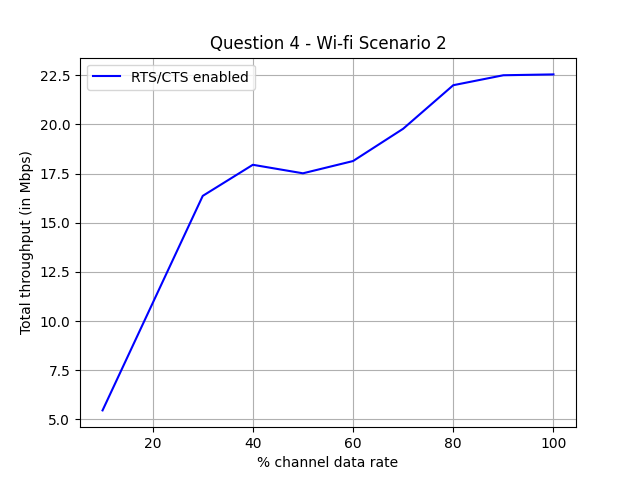
\includegraphics{q4.png}
\end{figure}

\begin{table}[H]
    \centering
    \begin{tabular}{||c|c||c|c||c||}
         \hline
         Total Data Rate Offered & \texttt{dataRate} & Flow 1 & Flow 2 & Total Throughput \\
         \hline % 10
         10\% of channel date rate & 2.7Mbps & 2.7296 Mbps & 2.7245 Mbps & 5.4541 Mbps \\
         \hline % 20
         20\% of channel date rate & 5.4Mbps & 5.4592 Mbps & 5.4516 Mbps & 10.9108 Mbps \\
         \hline % 30
         30\% of channel date rate & 8.1Mbps & 8.1888 Mbps & 8.1787 Mbps & 16.3675 Mbps \\
         \hline % 40
         40\% of channel date rate & 10.8Mbps & 7.0430 Mbps & 10.9032 Mbps & 17.9462 Mbps \\
         \hline % 50
         50\% of channel date rate & 13.5Mbps & 3.8856 Mbps & 13.6303 Mbps & 17.5159 Mbps \\
         \hline % 60
         60\% of channel date rate & 16.2Mbps & 1.7824 Mbps & 16.3573 Mbps & 18.1397 Mbps \\
         \hline % 70
         70\% of channel date rate & 18.9Mbps & 0.6977 Mbps & 19.0844 Mbps & 19.7821 Mbps \\
         \hline % 80
         80\% of channel date rate & 21.6Mbps & 0.1884 Mbps & 21.8090 Mbps & 21.9974 Mbps \\
         \hline % 90
         90\% of channel date rate & 24.3Mbps & 0.0331 Mbps & 22.4710 Mbps & 22.5041 Mbps \\
         \hline % 100
         100\% of channel date rate & 27.0Mbps & 0.0255 Mbps & 22.5219 Mbps & 22.5474 Mbps \\
         \hline         
    \end{tabular}
\end{table}

We can see that Total throughput increases with Offered Load and almost flattens to a constant value by the end with a minor dip in middle. \\

\subsection*{c.}
\addcontentsline{toc}{subsection}{c.}

\begin{itemize}
    \item Total throughput is less than total data rate offered.
    \item We can see that Total throughput increases with Offered Load and almost flattens to a constant value by the end with a minor dip in middle.
    \item We reach saturation when total data rate offered is about 80\% of channel data rate.
    \item The minor dip in the middle is due to more decrease in Flow 1 than increase in Flow 2.
    \item Throughputs of Flow 2 is more than Flow 1.
    \item For around till 30\%, we see that the collisions are negligible and all the flows are almost at peak (the linear growth).
    \item After that, we see a dip in Flow 1. This is due to increase in collisions (as \texttt{dataRate} is increased), Flow 2 over-powering Flow 1.
    \item This scenario was also part of CS 224 Midsem. Theoretically, I had shown that Flow 1 $<$ Flow 2.
    See \hyperref[Appendix 2]{Appendix 2}.
\end{itemize}

\newpage
\section*{Appendix 1}
\addcontentsline{toc}{section}{Appendix 1}
\label{Appendix 1}

\begin{figure}[H]
    \centering
    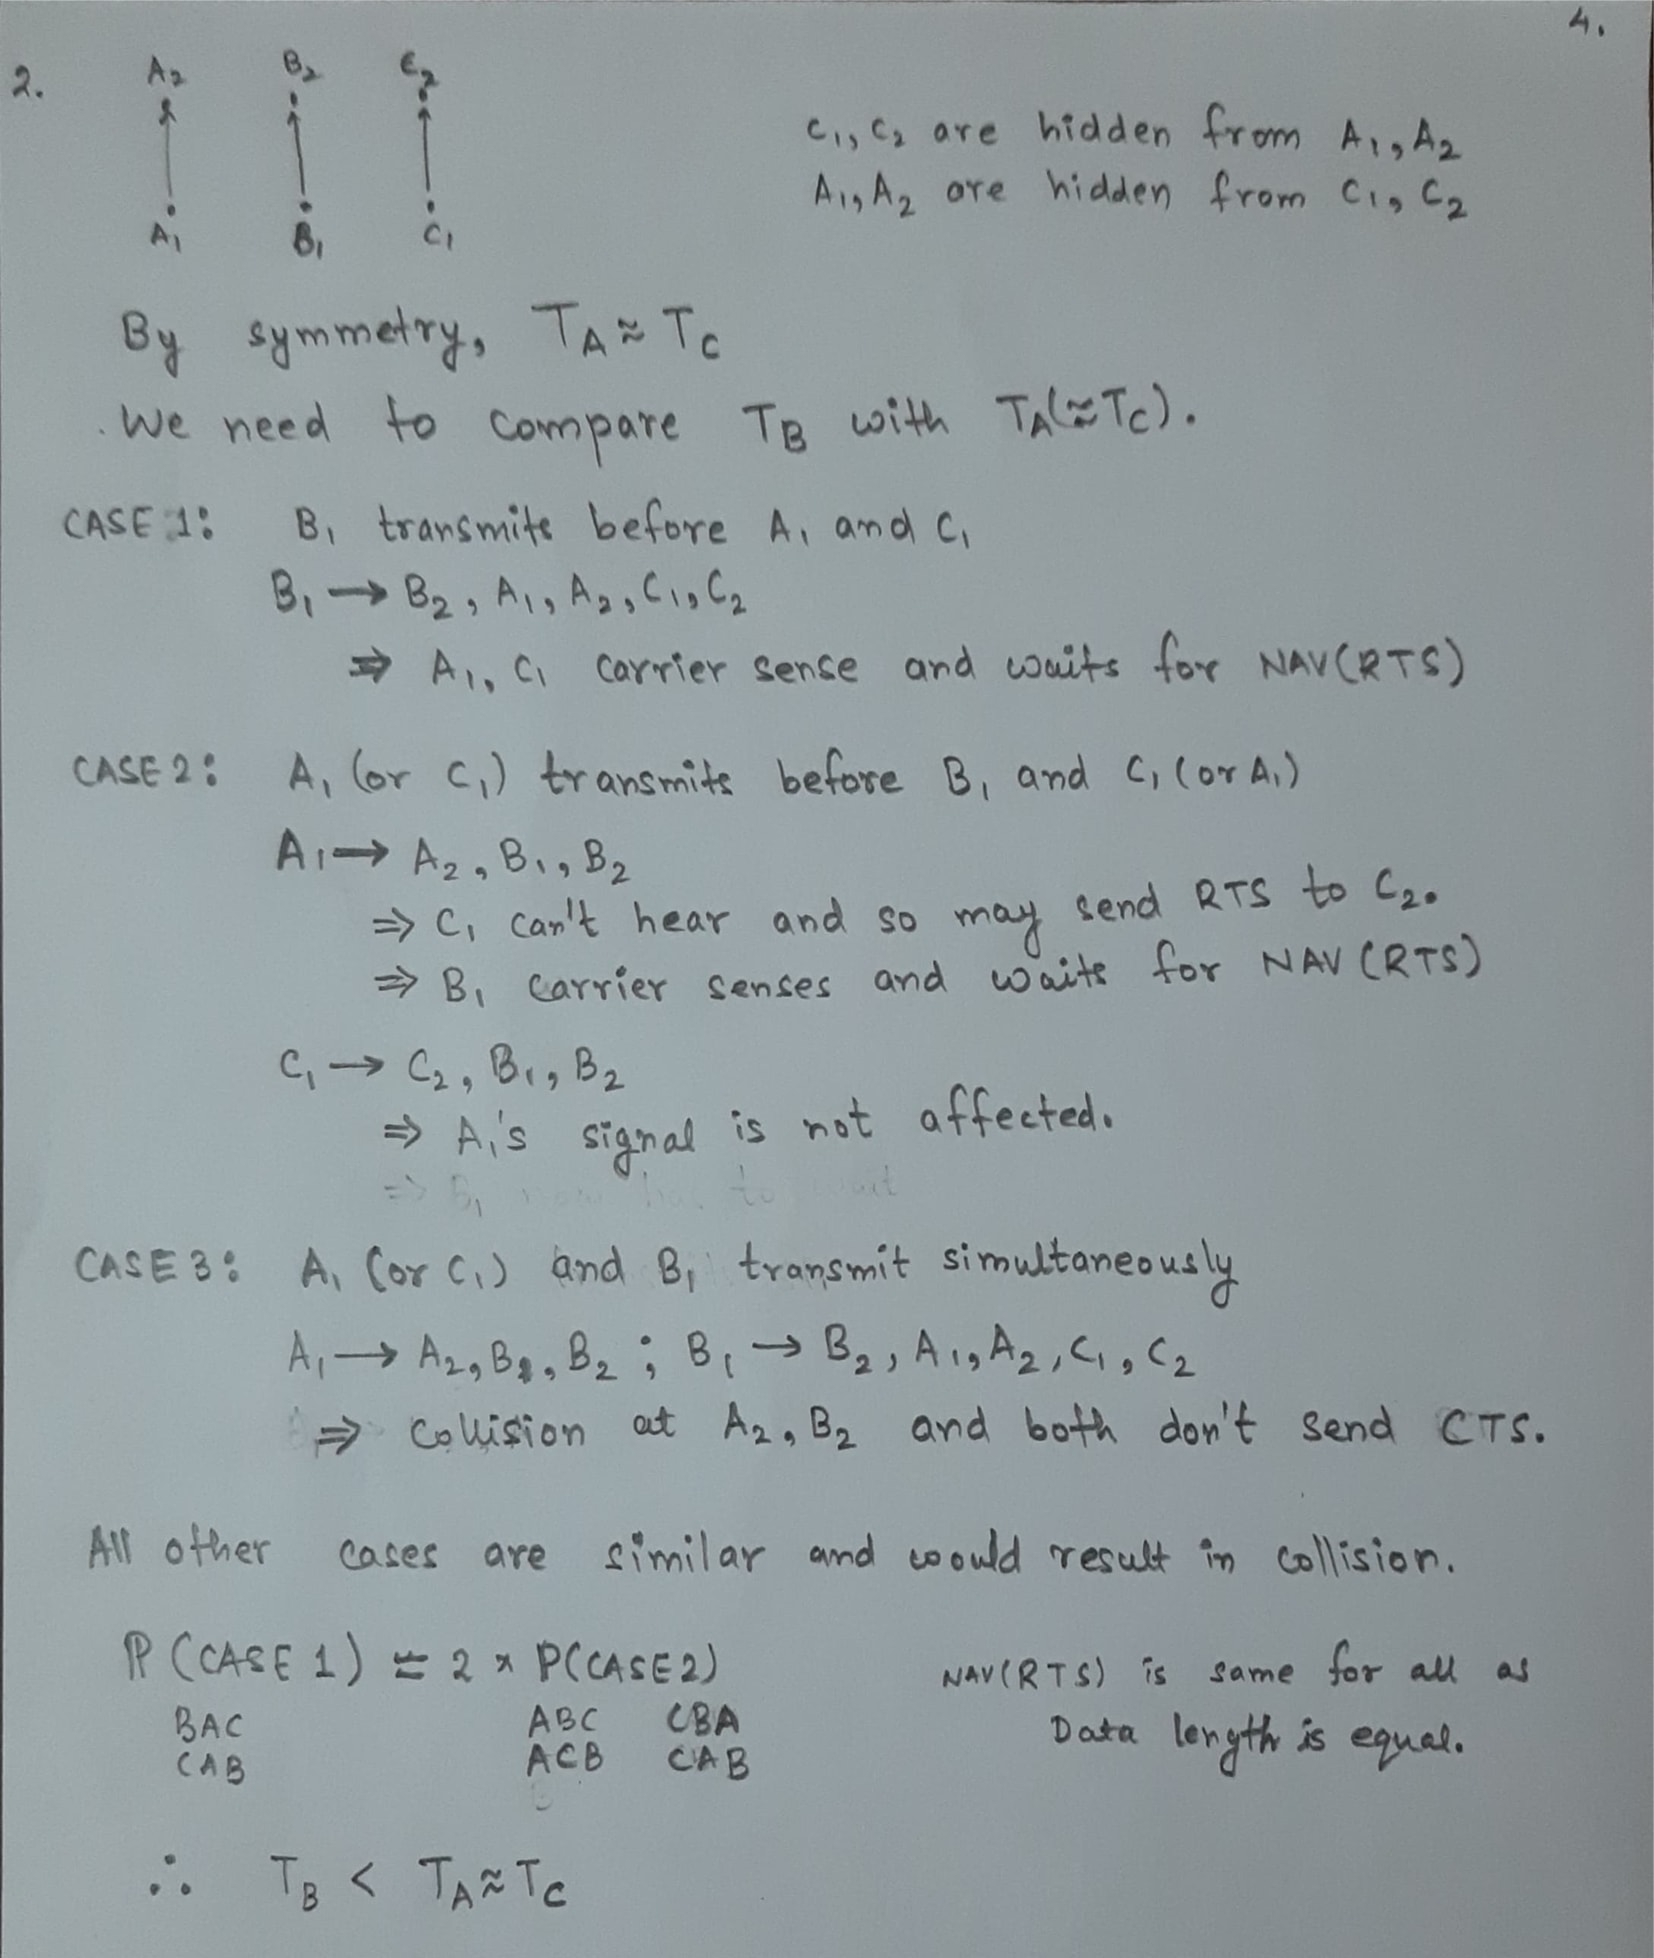
\includegraphics[scale=0.3]{Appendix_1.jpg}
\end{figure}

\newpage
\section*{Appendix 2}
\addcontentsline{toc}{section}{Appendix 2}
\label{Appendix 2}

\begin{figure}[H]
    \centering
    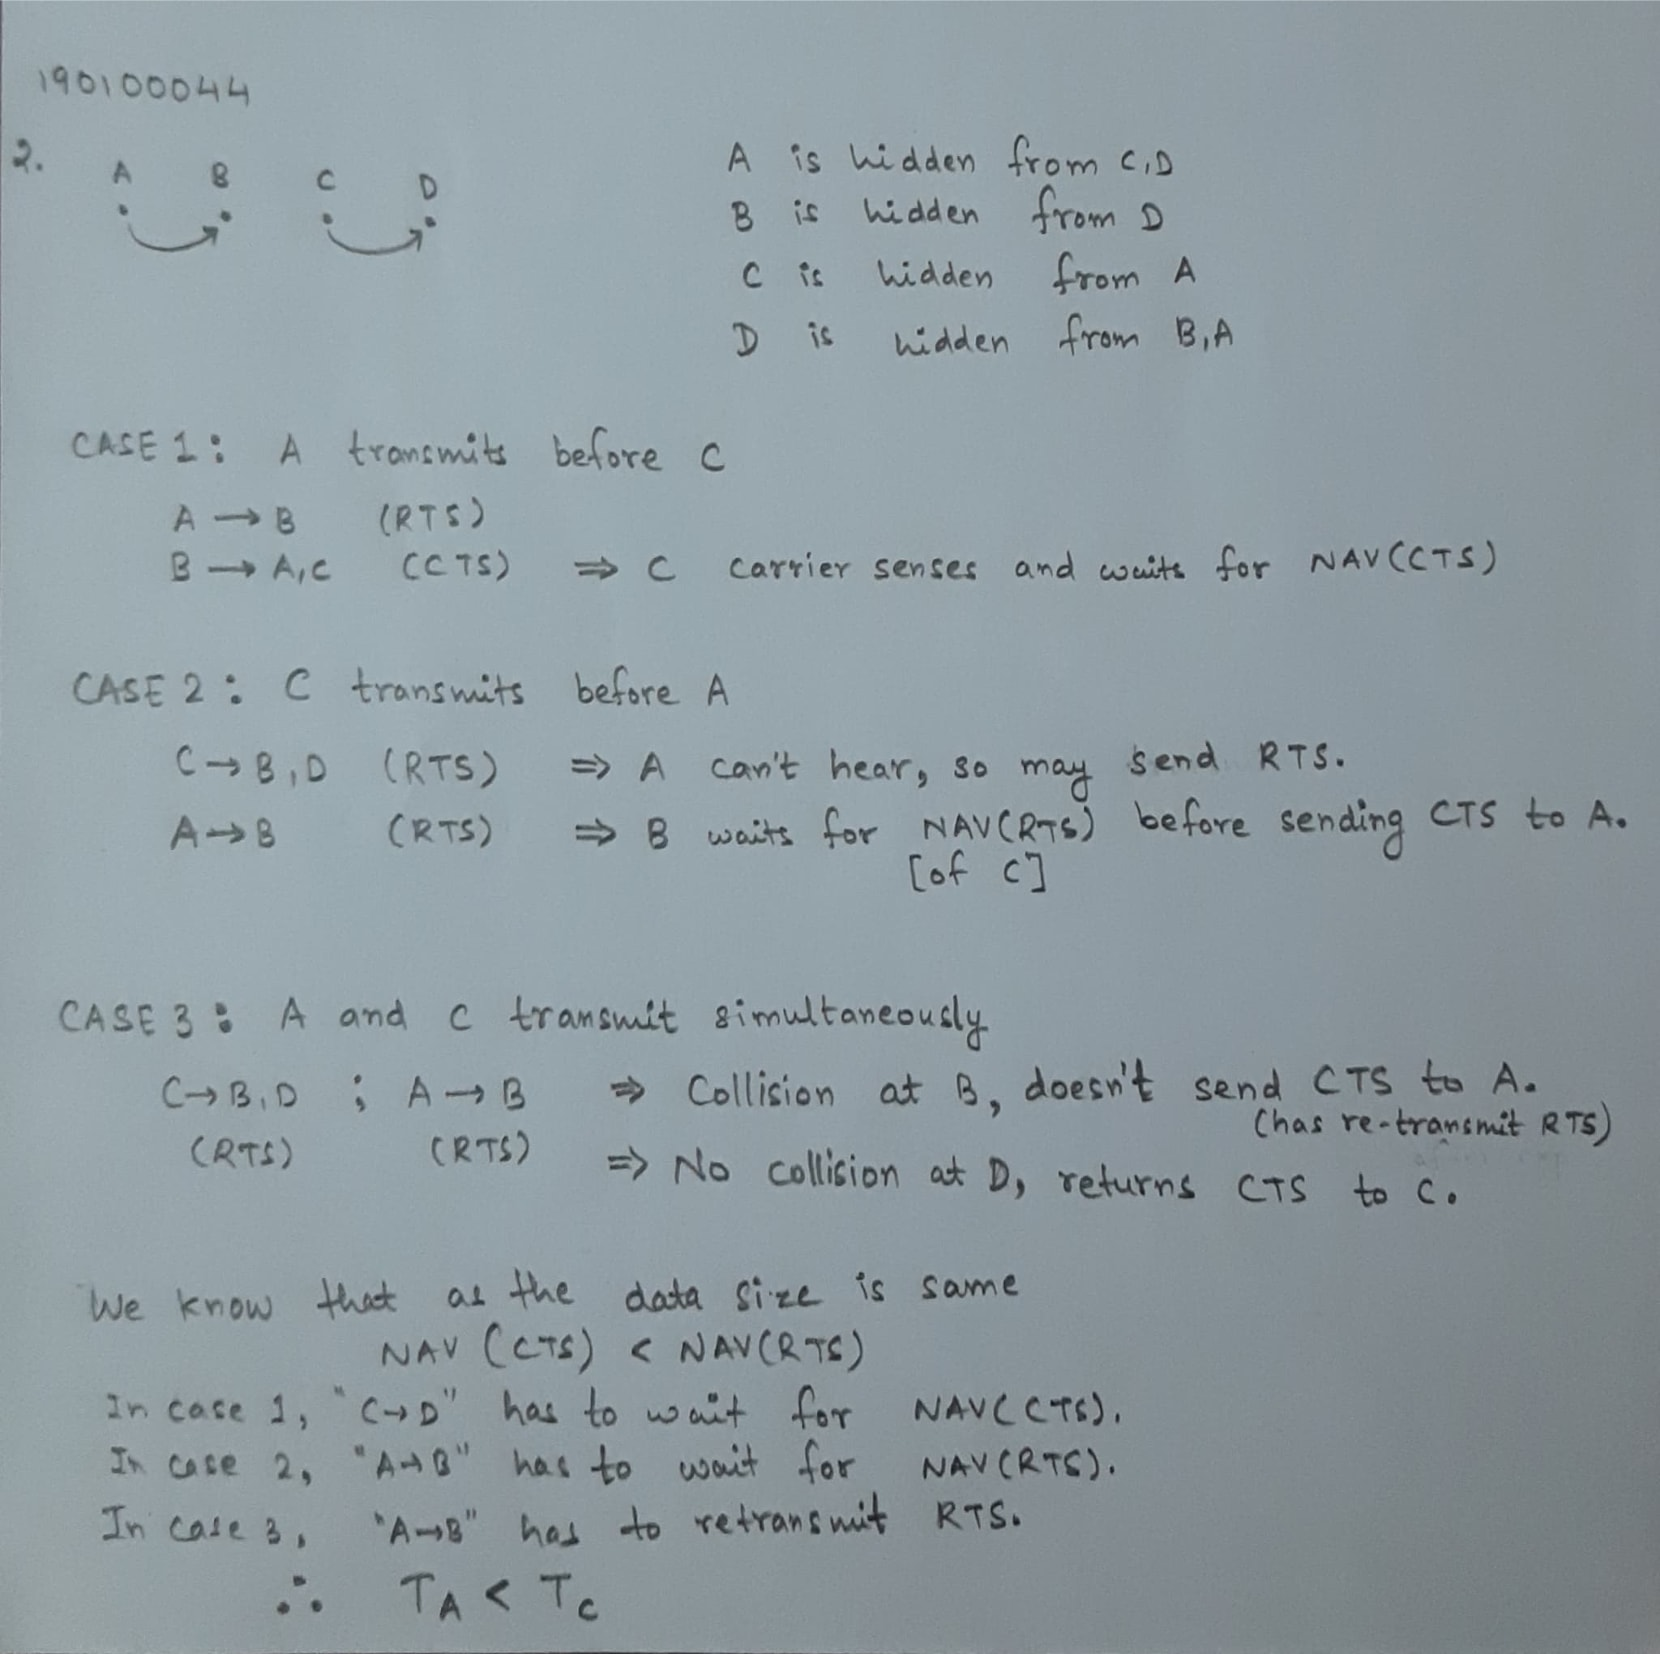
\includegraphics[scale=0.3]{Appendix_2.jpg}
\end{figure}

\end{document}
